\chapter{\TLAPlus 模型检查补充材料}
\label{appendix:tla-material}

\section{核心状态转换动作的\TLAPlus 源码}
\label{appendix:tla-actions}

正文 §4.2 以自然语言和数学符号说明了事务开始、操作执行、事务提交三类动作的语义。本节给出对应的 \TLAPlus 源码（经 \texttt{tla2tex} 排版，与原始 \texttt{MixedIsolation.tla} 模块中的写法一致），供需要核对形式化表达细节的读者参考。

\begin{figure}[htbp]
    \centering
    \includegraphics[width=0.95\textwidth]{figures/tla/Actions-crop.pdf}
    \caption{三类核心状态转换动作的 \TLAPlus 形式化定义}
    \label{fig:tla-actions}
\end{figure}

\section{SmallBank 负载测试用例}
\label{appendix:tla-smallbank}

\begin{center}
    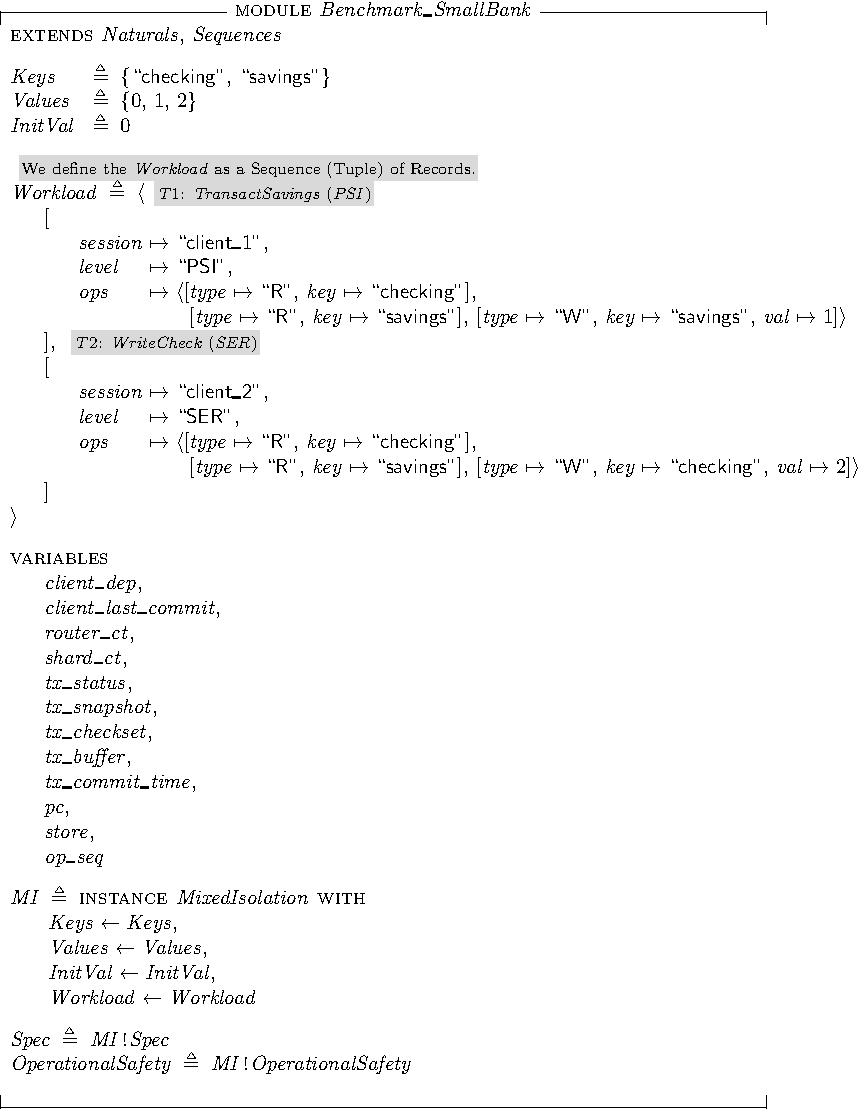
\includegraphics[width=0.9\textwidth]{figures/tla/Benchmark_SmallBank-crop.pdf}
    \captionof{figure}{SmallBank 负载测试用例}
    \label{fig:tla-smallbank}
\end{center}
